% Apresentar os passos e o código utilizado para calcular a FFT no Octave, incluindo detalhes como a janela temporal, se aplicável, e a normalização dos resultados.

% Considere o sinal \( x[n] = C + A \cos(2 \pi f_0 n T_s) \), onde:
% \begin{itemize}
%     \item \( C \) é a componente DC do sinal (amplitude da componente de frequência zero),
%     \item \( A \) é a amplitude da componente de cosseno,
%     \item \( f_0 = 100 \, \text{Hz} \) é a frequência do cosseno,
%     \item \( T_s = \frac{1}{f_s} = \frac{1}{1000} \) é o período de amostragem, com frequência de amostragem \( f_s = 1000 \, \text{Hz} \).
% \end{itemize}

% Substituindo \( T_s \) na expressão do sinal, temos:

% \[
% x[n] = C + A \cos \left( 2 \pi f_0 n \frac{1}{f_s} \right) = C + A \cos \left( 2 \pi \frac{f_0}{f_s} n \right)
% \]

% Como \( f_0 = 100 \, \text{Hz} \) e \( f_s = 1000 \, \text{Hz} \), obtemos:

% \[
% \frac{f_0}{f_s} = \frac{100}{1000} = 0.1
% \]

% Portanto,

% \[
% x[n] = C + A \cos (2 \pi \cdot 0.1 \cdot n) = C + A \cos (0.2 \pi n)
% \]

% \subsection*{Cálculo da DTFT}

% A DTFT do sinal \( x[n] = C + A \cos(0.2 \pi n) \) pode ser obtida calculando a DTFT de cada termo separadamente.

% \subsubsection*{1. DTFT da Componente DC \( C \)}

% A componente DC, \( C \), tem uma DTFT que é um impulso em \( \omega = 0 \):

% \[
% X_{\text{DC}}(e^{j \omega}) = C \cdot 2 \pi \delta(\omega)
% \]

% \subsubsection*{2. DTFT da Componente Cossenoidal \( A \cos(0.2 \pi n) \)}

% Podemos expressar o cosseno em termos de exponenciais complexas:

% \[
% A \cos(0.2 \pi n) = \frac{A}{2} \left( e^{j 0.2 \pi n} + e^{-j 0.2 \pi n} \right)
% \]

% A DTFT de \( e^{j 0.2 \pi n} \) é um impulso em \( \omega = 0.2 \pi \), e a DTFT de \( e^{-j 0.2 \pi n} \) é um impulso em \( \omega = -0.2 \pi \):

% \[
% X_{\cos}(e^{j \omega}) = \frac{A}{2} \cdot 2 \pi \left( \delta(\omega - 0.2 \pi) + \delta(\omega + 0.2 \pi) \right)
% \]

% \subsubsection*{3. DTFT do Sinal Total \( x[n] \)}

% Somando as duas DTFTs, obtemos:

% \[
% X(e^{j \omega}) = C \cdot 2 \pi \delta(\omega) + \frac{A}{2} \cdot 2 \pi \left( \delta(\omega - 0.2 \pi) + \delta(\omega + 0.2 \pi) \right)
% \]

% Simplificando:

% \[
% X(e^{j \omega}) = 2 \pi \left( C \delta(\omega) + \frac{A}{2} \delta(\omega - 0.2 \pi) + \frac{A}{2} \delta(\omega + 0.2 \pi) \right)
% \]



% Consideramos um sinal genérico dado por:
% \[
% x[n] = C + A \cos(2 \pi f_0 n T_s)
% \]
% onde:
% \begin{itemize}
%     \item \( C \) é a componente DC (constante) do sinal,
%     \item \( A \) é a amplitude da componente cossenoidal,
%     \item \( f_0 \) é a frequência da componente cossenoidal,
%     \item \( T_s = \frac{1}{f_s} \) é o período de amostragem, onde \( f_s \) é a frequência de amostragem.
% \end{itemize}

% Para simplificar, substituímos \( T_s = \frac{1}{f_s} \) e reescrevemos o sinal como:

% \[
% x[n] = C + A \cos \left( 2 \pi \frac{f_0}{f_s} n \right)
% \]

% Definimos \( f_0 / f_s = \alpha \), que representa a frequência normalizada do cosseno, obtendo:

% \[
% x[n] = C + A \cos(2 \pi \alpha n)
% \]



Quando aplicamos uma janela \( w[n] \) ao sinal, o sinal janelado é dado por:
\[
x_w[n] = x[n] \cdot w[n]
\]
onde \( w[n] \) é uma função de janela de tamanho \( N \), usada para minimizar os efeitos de vazamento espectral. Exemplos comuns de janelas incluem a janela de Hamming, Hann, e retangular.

A DTFT do sinal janelado, \( X_w(e^{j \omega}) \), é dada pela convolução da DTFT do sinal original \( X(e^{j \omega}) \) com a DTFT da janela \( W(e^{j \omega}) \):
\[
X_w(e^{j \omega}) = X(e^{j \omega}) * W(e^{j \omega})
\]

\subsection*{DTFT do Sinal Sem Janela}

Para referência, a DTFT do sinal original \( x[n] = C + A \cos(2 \pi \alpha n) \) (sem janela) pode ser calculada como a soma das DTFTs de cada termo:

1. \textbf{DTFT da componente DC} \( C \):
   \[
   X_{\text{DC}}(e^{j \omega}) = C \cdot 2 \pi \delta(\omega)
   \]

2. \textbf{DTFT da componente cossenoidal} \( A \cos(2 \pi \alpha n) \):

   Podemos expressar o cosseno em termos de exponenciais complexas:
   \[
   A \cos(2 \pi \alpha n) = \frac{A}{2} \left( e^{j 2 \pi \alpha n} + e^{-j 2 \pi \alpha n} \right)
   \]
   Assim, a DTFT dessa parte é:
   \[
   X_{\cos}(e^{j \omega}) = \frac{A}{2} \cdot 2 \pi \left( \delta(\omega - 2 \pi \alpha) + \delta(\omega + 2 \pi \alpha) \right)
   \]

3. \textbf{DTFT do sinal total} \( x[n] \):
   \[
   X(e^{j \omega}) = C \cdot 2 \pi \delta(\omega) + \frac{A}{2} \cdot 2 \pi \left( \delta(\omega - 2 \pi \alpha) + \delta(\omega + 2 \pi \alpha) \right)
   \]

\subsection*{DTFT do Sinal Janelado}

Quando a janela \( w[n] \) é aplicada, o espectro do sinal janelado \( X_w(e^{j \omega}) \) é a convolução do espectro do sinal \( X(e^{j \omega}) \) com o espectro da janela \( W(e^{j \omega}) \):
\[
X_w(e^{j \omega}) = X(e^{j \omega}) * W(e^{j \omega})
\]

\subsection*{Computacionalmente}
No Octave, aplicamos a função da FFT para obter uma aproximação da DTFT, como mostra o exemplo abaixo.

\lstinputlisting[language=Octave]{02_analytic_development/example_fft.m}
\begin{figure}[H]
    \centering
    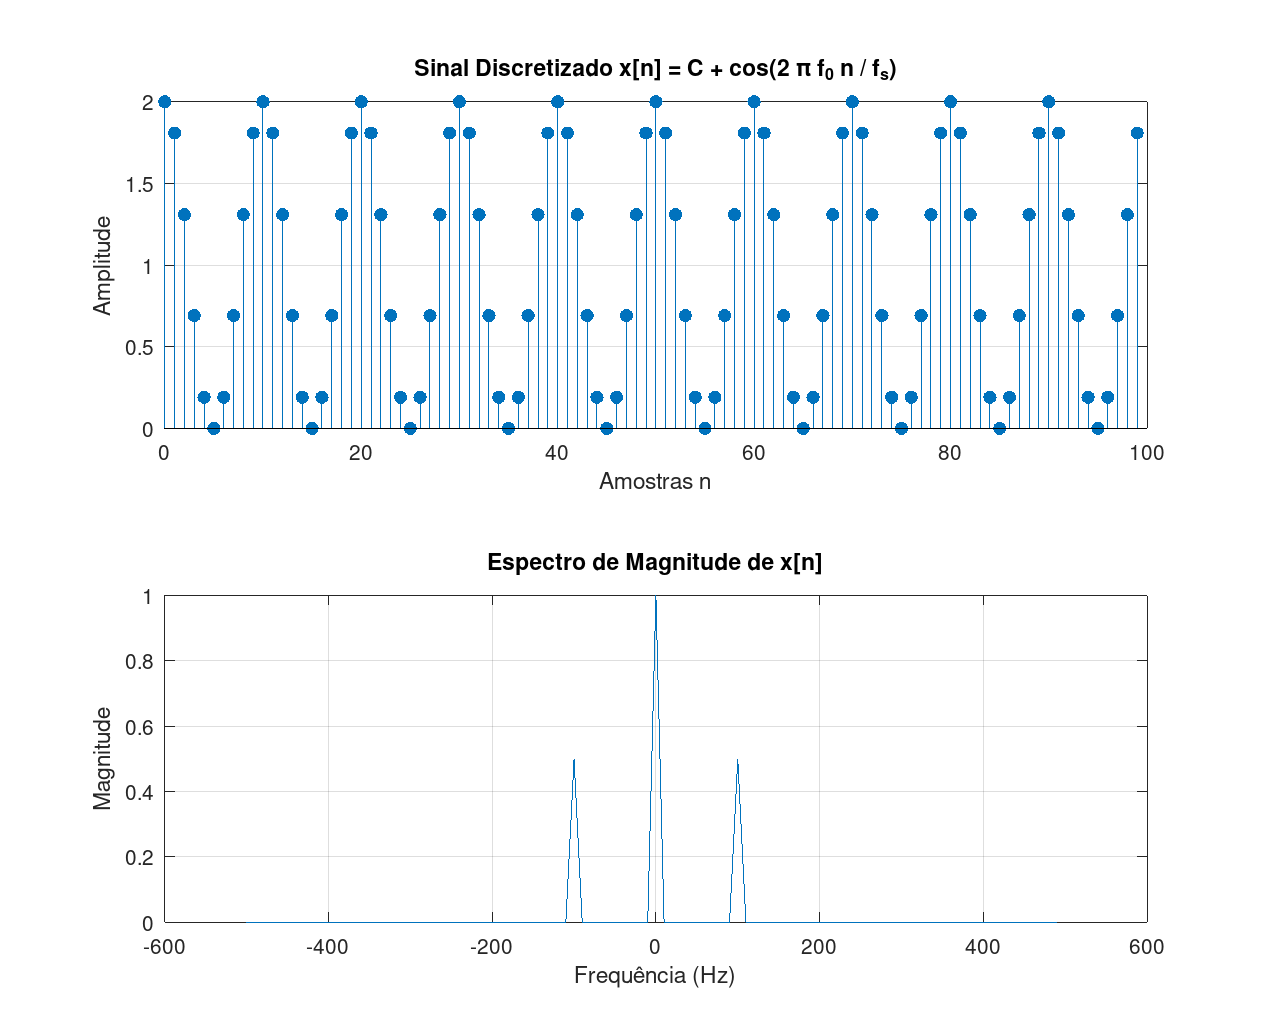
\includegraphics[width=1\linewidth]{02_analytic_development/example_fft.png}
    \caption{Sinal e Espectro de Magnitude}
    \label{fig:enter-label}
\end{figure}